## Tipos de dato lógico

- Hasta ahora hemos visto variables numéricas, y en menor medida, de texto.

- He aquí un nuevo tipo de dato, muy sencillo:

\pause

\bgnblockdefinition
\bld{Tipo de dato lógico:} corresponden a la respuesta a preguntas lógicas, donde las
únicas opciones son\newline \structure{True} o \structure{False}.
\trmblockdefinition

\vspace{.6ex}

\scalebox{.7}{%
\begin{tikzpicture}[every node/.style={cloud callout, draw, fill=Wheat1!50, cloud ignores aspect, cloud puffs=12, text width=5em, text centered}]
\node at (0,0) {\bf ¿Es $n$ positivo?};
\node at (4,1) {\bf ¿Está el producto en oferta?};
\node at (8,-1) {\bf ¿Es el vuelto > 0?};
\node at (12,0) {\bf ¿Quedan elementos en la lista?};
\end{tikzpicture}
}

## Tipos de dato lógico: {.fragile}

\simpleTitle{Los operadores condicionales más importantes son:}

\begin{zebraTable}[0.5]%
    \rowcolor{structure}%
    \textcolor{white}{Operador} & \textcolor{white}{Significado} \\
    \nzinlinecode{==} &  Igualdad \\
    \nzinlinecode{!=} & Diferentes \\
    \nzinlinecode{not} &  Negación \\
    \nzinlinecode{<} &  Menor que \\
    \nzinlinecode{>} &  Mayor que \\
    \nzinlinecode{<=} & Menor o igual que \\
    \nzinlinecode{>=} & Mayor o igual que \\
    \nzinlinecode{and} &  Y \\
    \nzinlinecode{or} &   O \\
\end{zebraTable}


## Tipos de dato lógico: {.fragile}

\simpleTitle{Probemos algunas expresiones en Python:}

\vspace{-3ex}

\bgncolumns

\column{0.35\textwidth}

\begin{lstlisting}
>>> 7 < 10
True

>>> 8 < 2
False

>>> 8 > 4
True

>>> 8 > 11
False

>>> 4 > 4
False
\end{lstlisting}

\column{0.35\textwidth}

\begin{lstlisting}
>>> 3 == 6
False

>>> 6 == 3 * 2
True

>>> 10 != 7
True

>>> 8 <= 10
True

>>> 10 >= 3**2
True
\end{lstlisting}

\column{0.35\textwidth}

\begin{lstlisting}
>>> True == True
True

>>> False == True
False

>>> False == False
True
\end{lstlisting}

\trmcolumns


## Tipos de dato lógico: {.fragile}

\simpleTitle{Probemos algunas expresiones con variables:}

\vspace{-3ex}

\bgncolumns

\column{0.35\textwidth}

\begin{lstlisting}
>>> largo = 12
>>> ancho = 7
>>> alto = 6
>>> listo = True
>>> suficiente = 90

>>> largo > ancho
True

>>> largo < 2 * ancho
True

>>> alto == largo / 2
True
\end{lstlisting}

\column{0.65\textwidth}

\begin{lstlisting}
>>> alto <= largo
True

>>> alto * ancho < largo
False

>>> listo (*@\tikzmark{bgnSetbool}@*)= (largo * ancho) > suficiente
>>> listo
False

>>> listo (*@\tikzmark{trmSetbool}@*)= (1.2*largo * ancho) > suficiente
>>> listo
True
\end{lstlisting}

\trmcolumns

\drawTikZComment[below right=2em and 3em of trmSetbool]{trmSetbool}{\scriptsize Se puede asignar un resultado lógico}
\drawTikZAnotherArrow{bgnSetbool}{trmSetbool-comment}

## Tipos de dato lógico: {.fragile}

\simpleTitle{Probemos algunas expresiones compuestas:}

\begin{lstlisting}
>>> (1.2*largo * ancho) > suficiente and alto > 5
True

>>> listo and alto > 5
True

>>> listo = largo > 10 and ancho <= 6
>>> listo
False

>>> listo = largo > 10 or ancho <= 6
>>> listo
True

>>> not (largo > 10 or ancho <= 6)
False
\end{lstlisting}

## Funciones booleanas {.fragile}

- Una función también puede retornar un tipo lógico:

\begin{lstlisting}
# esPar: int -> bool(*@\tikzmark{booltypedesign01}@*)
# Si 'numero' es par, retorna verdadero;
# en caso contrario retorna False.
# Ejemplo: esPar(7) retorna False
def esPar(numero):
    return (numero % 2) == 0

# Test
assert esPar(2) == True
assert esPar(11) == False
\end{lstlisting}

\pause

\drawTikZComment[right=8em of booltypedesign01]{booltypedesign01}{\scriptsize Nuevo tipo de dato en nuestra receta}

## Funciones booleanas {.fragile}

- Una función también puede retornar un tipo lógico:

\begin{lstlisting}
# esMultiploDe: int int -> bool(*@\tikzmark{booltypedesign02}@*)
# Si 'numero' es múltiplo de 'factor', retorna verdadero;
# en caso contrario retorna False.
# Ejemplo: esMultiploDe(7, 3) retorna False
def esMultiploDe(numero, factor):
    return (numero % factor) == 0

# Test
assert esMultiploDe(21, 7) == True
assert esMultiploDe(18, 5) == False
\end{lstlisting}

## Condiciones {.fragile}

- La programación no se compone sólo\newline de cálculos.

\begin{tikzpicture}[remember picture, overlay]
    \tikzSign[turnleft,turnright]{12mm}{a1}{$(current page.north east)+(-20mm,-28mm)$}
\end{tikzpicture} 

\vspace{-.6ex}

\pause

\bgnblockidea
Muchas veces debemos \strongText{tomar decisiones}.
\trmblockidea

\vspace{2ex}

Ejemplos:

- ¿Cuál es el mayor entre dos números?
- ¿Debo dar vuelto?
- ¿Es martes hoy?
- ¿La temperatura actual es mayor o igual a 30°C?

## Condiciones {.fragile}

\simpleTitle{Ejemplo:}

- Le pedimos un número al usuario.
- Debemos determinar si ese número es mayor que cero.

\bgnblocknormal[wd=.8\textwidth,centered]
Escribiremos todo el código dentro de un módulo de Python.
\trmblocknormal

\tikz[remember picture, overlay]{\tikzSign[turnleft,keepstraight]{12mm}{a1}{$(current page.north east)+(-20mm,-28mm)$}}

\pause

\bgncolumns
\column{.55\textwidth}
\vspace{-1ex}
\simpleTitle{Código:}

\begin{lstlisting}
num = input('Ingrese un número: ')

if num > 0:
    print('Es mayor que cero.')
else:
    print('No es mayor que cero.')
\end{lstlisting}

\column{.05\textwidth}
\column{.4\textwidth}
\vspace{-1ex}
\simpleTitle{Ejecución:}

\begin{exampleConsole}
Ingrese un número: \codeInput{23}
Es mayor que cero.
\end{exampleConsole}

\trmcolumns


## Condiciones {.fragile}

\tikz[remember picture, overlay]{\tikzSign[keepstraight,turnright]{8mm}{a1}{$(current page.north east)+(-16mm,-20mm)$}}
\vspace{-3ex}

\bgncolumns
\column{.55\textwidth}
\vspace{-1ex}

\simpleTitle{Código:}

\begin{lstlisting}
num = input('Ingrese un número: ')

if num > 0:
    print('Es mayor que cero.')
else:
    print('No es mayor que cero.')
\end{lstlisting}

\only{<2->}{%
    \vspace{2ex}

    \bgnblockidea
    Construyamos ahora una función que haga esto mismo.
    \trmblockidea
}

\column{.05\textwidth}
\column{.4\textwidth}
\vspace{-1ex}

\simpleTitle*{Ejecución 1:}

\begin{exampleConsole}
Ingrese un número: \codeInput{23}
Es mayor que cero.
\end{exampleConsole}

\fullrule

\simpleTitle*{Ejecución 2:}

\begin{exampleConsole}
Ingrese un número: \codeInput{-1}
No es mayor que cero.
\end{exampleConsole}

\fullrule

\simpleTitle*{Ejecución 3:}

\begin{exampleConsole}
Ingrese un número: \codeInput{0}
No es mayor que cero.
\end{exampleConsole}

\trmcolumns

## Condiciones {.fragile}

\begin{lstlisting}
# esMayorQueCero: int -> None(*@\tikzmark{nonetypedesign01}@*)
# Recibe un número entero, e imprime en
# pantalla un mensaje avisando si ese
# número es mayor que cero, o no.
# Ejemplo: esMayorQueCero(23)
def esMayorQueCero(num):
    if num > 0:
        print('Es mayor que cero.')
    else:
        print('No es mayor que cero.')
\end{lstlisting}

\tikz[remember picture, overlay]{\tikzSign[turnleft,turnright]{8mm}{a1}{$(current page.north east)+(-16mm,-20mm)$}}
\vspace{-3ex}

\pause

\drawTikZComment[below right=.2em and 7em of nonetypedesign01]{nonetypedesign01}{\scriptsize Nuevo tipo de dato en nuestra receta: se usa cuando no se retorna nada.}
\vspace{-3ex}

\pause


\bgncolumns
\column{.55\textwidth}
\vspace{-1ex}

\simpleTitle{Código:}

\begin{lstlisting}
# Ahora usamos la función: 
num = input('Ingrese un número: ')
esMayorQueCero(num)
\end{lstlisting}

\column{.05\textwidth}
\column{.4\textwidth}
\vspace{-1ex}

\simpleTitle*{Ejecución:}

\begin{exampleConsole}
Ingrese un número: \codeInput{11}
Es mayor que cero.
\end{exampleConsole}

\trmcolumns

## Condiciones {.fragile}

\simpleTitle{Otro ejemplo:}

\tikz[remember picture, overlay]{\tikzSign[turnleft,keepstraight]{8mm}{a1}{$(current page.north east)+(-16mm,-20mm)$}}
\vspace{-3ex}

- Dados dos números, determinar cuál es el mayor.

\vspace{-1ex}
\begin{lstlisting}
# imprimeElMayor: int int -> None
# Recibe dos números, e indica en pantalla cuál es el mayor.
# Ejemplo: imprimeElMayor(11, 3)
def imprimeElMayor(numA, numB):
    if numA > numB:(*@\tikzmark{nottestingequal}@*)
        print('El mayor es: ' + str(numA))
    else:
        print('El mayor es: ' + str(numB))
\end{lstlisting}

\vspace{-2ex}

\bgncolumns
\column{.55\textwidth}

\simpleTitle{Código:}

\begin{lstlisting}
num1 = input('Ingrese un número: ')
num2 = input('Ingrese otro número: ')
imprimeElMayor(num1, num2)
\end{lstlisting}

\column{.45\textwidth}

\simpleTitle*{Ejecución:}

\begin{exampleConsole}
Ingrese un número: \codeInput{5}
Ingrese otro número: \codeInput{3}
El mayor es: 5
\end{exampleConsole}

\trmcolumns

\pause

\drawTikZComment[right=10em of nottestingequal, text width=30mm]{nottestingequal}{\scriptsize No detectamos cuando son iguales...}
\vspace{-3ex}


## Condiciones {.fragile}

\simpleTitle{Otro ejemplo:}

\tikz[remember picture, overlay]{\tikzSign[keepstraight,turnright]{8mm}{a1}{$(current page.north east)+(-16mm,-20mm)$}}
\vspace{-3ex}

- Dados dos números, determinar cuál es el mayor.
    - \alert{Destacar cuando sean iguales.}

\begin{lstlisting}
# imprimeElMayorOIgual: int int -> None
# Recibe dos números, e indica en pantalla cuál es el mayor,
# o avisa cuando son iguales.
# Ejemplo: imprimeElMayorOIgual(11, 3)
def imprimeElMayorOIgual(numA, numB):
    if numA > numB:
        print('El mayor es: ' + str(numA))
    elif numA < numB:
        print('El mayor es: ' + str(numB))
    else:
        print('Los dos números son iguales.')
\end{lstlisting}

## Condiciones {.fragile}

\tikz[remember picture, overlay]{\tikzSign[turnleft,turnright]{8mm}{a1}{$(current page.north east)+(-16mm,-20mm)$}}
\vspace{-3ex}

\bgncolumns
\column{.52\textwidth}
\vspace{-1ex}

\simpleTitle{Código:}

\begin{lstlisting}
num1 = input('Ingrese un número: ')
num2 = input('Ingrese otro: ')
imprimeElMayorOIgual(num1, num2)
\end{lstlisting}

\column{.48\textwidth}
\vspace{-1ex}

\simpleTitle*{Ejecución 1:}

\begin{exampleConsole}
Ingrese un número: \codeInput{2}
Ingrese otro: \codeInput{7}
El mayor es: 7
\end{exampleConsole}

\fullrule

\simpleTitle*{Ejecución 2:}

\begin{exampleConsole}
Ingrese un número: \codeInput{4}
Ingrese otro: \codeInput{4}
Los dos números son iguales.
\end{exampleConsole}

\trmcolumns
